\documentclass[pdftex,a4paper,12pt]{report}

\usepackage[utf8]{inputenc}  % Accenten gebruiken in tekst (vb. é ipv \'e)
\usepackage{amsfonts}        % AMS math packages: extra wiskundige
\usepackage{amsmath}         %   symbolen (o.a. getallen-
\usepackage{amssymb}         %   verzamelingen N, R, Z, Q, etc.)
\usepackage[dutch]{babel}    % Taalinstellingen: woordsplitsingen,
                             %  commando's voor speciale karakters
                             %  ("dutch" voor NL)
\usepackage{eurosym}         % Euro-symbool €
\usepackage{geometry}
\usepackage{graphicx}        % Invoegen van tekeningen
\usepackage[pdftex,bookmarks=true]{hyperref}
                             % PDF krijgt klikbare links & verwijzingen,
                             %  inhoudstafel
\usepackage{listings}        % Broncode mooi opmaken
\usepackage{multirow}        % Tekst over verschillende cellen in tabellen
\usepackage{rotating}        % Tabellen en figuren roteren
\usepackage{natbib}          % Betere bibliografiestijlen
\usepackage{fancyhdr}        % Pagina-opmaak met hoofd- en voettekst

\usepackage[T1]{fontenc}     % Ivm lettertypes
\usepackage{lmodern}
\usepackage{textcomp}

\usepackage{lipsum}          % Voor vultekst (lorem ipsum)

%%---------- Layout ------------------------------------------------------

% hoofdingen, enz.
\pagestyle{fancy}
% enkel hoofdstuktitel in hoofding, geen sectietitel (vermijd overlap)
\renewcommand{\sectionmark}[1]{}

% lijn, wordt gebruikt in titelpagina
\newcommand{\HRule}{\rule{\linewidth}{0.5mm}}

% Leeg blad
\newcommand{\emptypage}{
\newpage
\thispagestyle{empty}
\mbox{}
\newpage
}

% Gebruik een schreefloos lettertype ipv het "oubollig" uitziende
% Computer Modern
\renewcommand{\familydefault}{\sfdefault}

% Commando voor invoegen Java-broncodebestanden (dank aan Niels Corneille)
% Gebruik: \codefragment{source/MijnKlasse.java}{Uitleg bij de code}
\newcommand{\codefragment}[2]{ \lstset{%
  language=java,
  breaklines=true,
  float=th,
  caption={#2},
  basicstyle=\scriptsize,
  frame=single,
  extendedchars=\true
}
\lstinputlisting{#1}}

%%---------- Documenteigenschappen ---------------------------------------
%% Vul dit aan met je eigen info:

% Je eigen naam
\newcommand{\student}{Nathan Baele}

% De naam van je lector, begeleider, promotor
\newcommand{\promotor}{Bert Van Vreckem}

% De naam van je co-promotor
\newcommand{\copromotor}{Selami Top}

% Indien je bachelorproef in opdracht van een bedrijf of organisatie
% geschreven is, geef je hier de naam.
\newcommand{\instelling}{---}

% De titel van het rapport/bachelorproef
\newcommand{\titel}{De efficiëntste manier om een Windows Server 2012 R2 netwerk te beveiligen tegen interne en externe bedreigingen in het bedrijfsleven}

% Datum van indienen
\newcommand{\datum}{29 mei 2015}

% Faculteit
\newcommand{\faculteit}{Faculteit Bedrijf en Organisatie}

% Soort rapport
\newcommand{\rapporttype}{Scriptie voorgedragen tot het bekomen van de graad van\\Bachelor in de toegepaste informatica}

% Academiejaar
\newcommand{\academiejaar}{2014-2015}

% Examenperiode
%  - 1e semester = 1e examenperiode
%  - 2e semester = 2e examenperiode
%  - tweede zit = 3e examenperiode
\newcommand{\examenperiode}{Tweede examenperiode}

%%========================================================================
%% Inhoud document
%%========================================================================

\begin{document}

%%---------- Front matter ------------------------------------------------
%% Het voorblad - Hier moet je in principe niets wijzigen.

\begin{titlepage}
  \newgeometry{top=2cm,bottom=1.5cm,left=1.5cm,right=1.5cm}
  \begin{center}

    \begingroup
    \rmfamily
    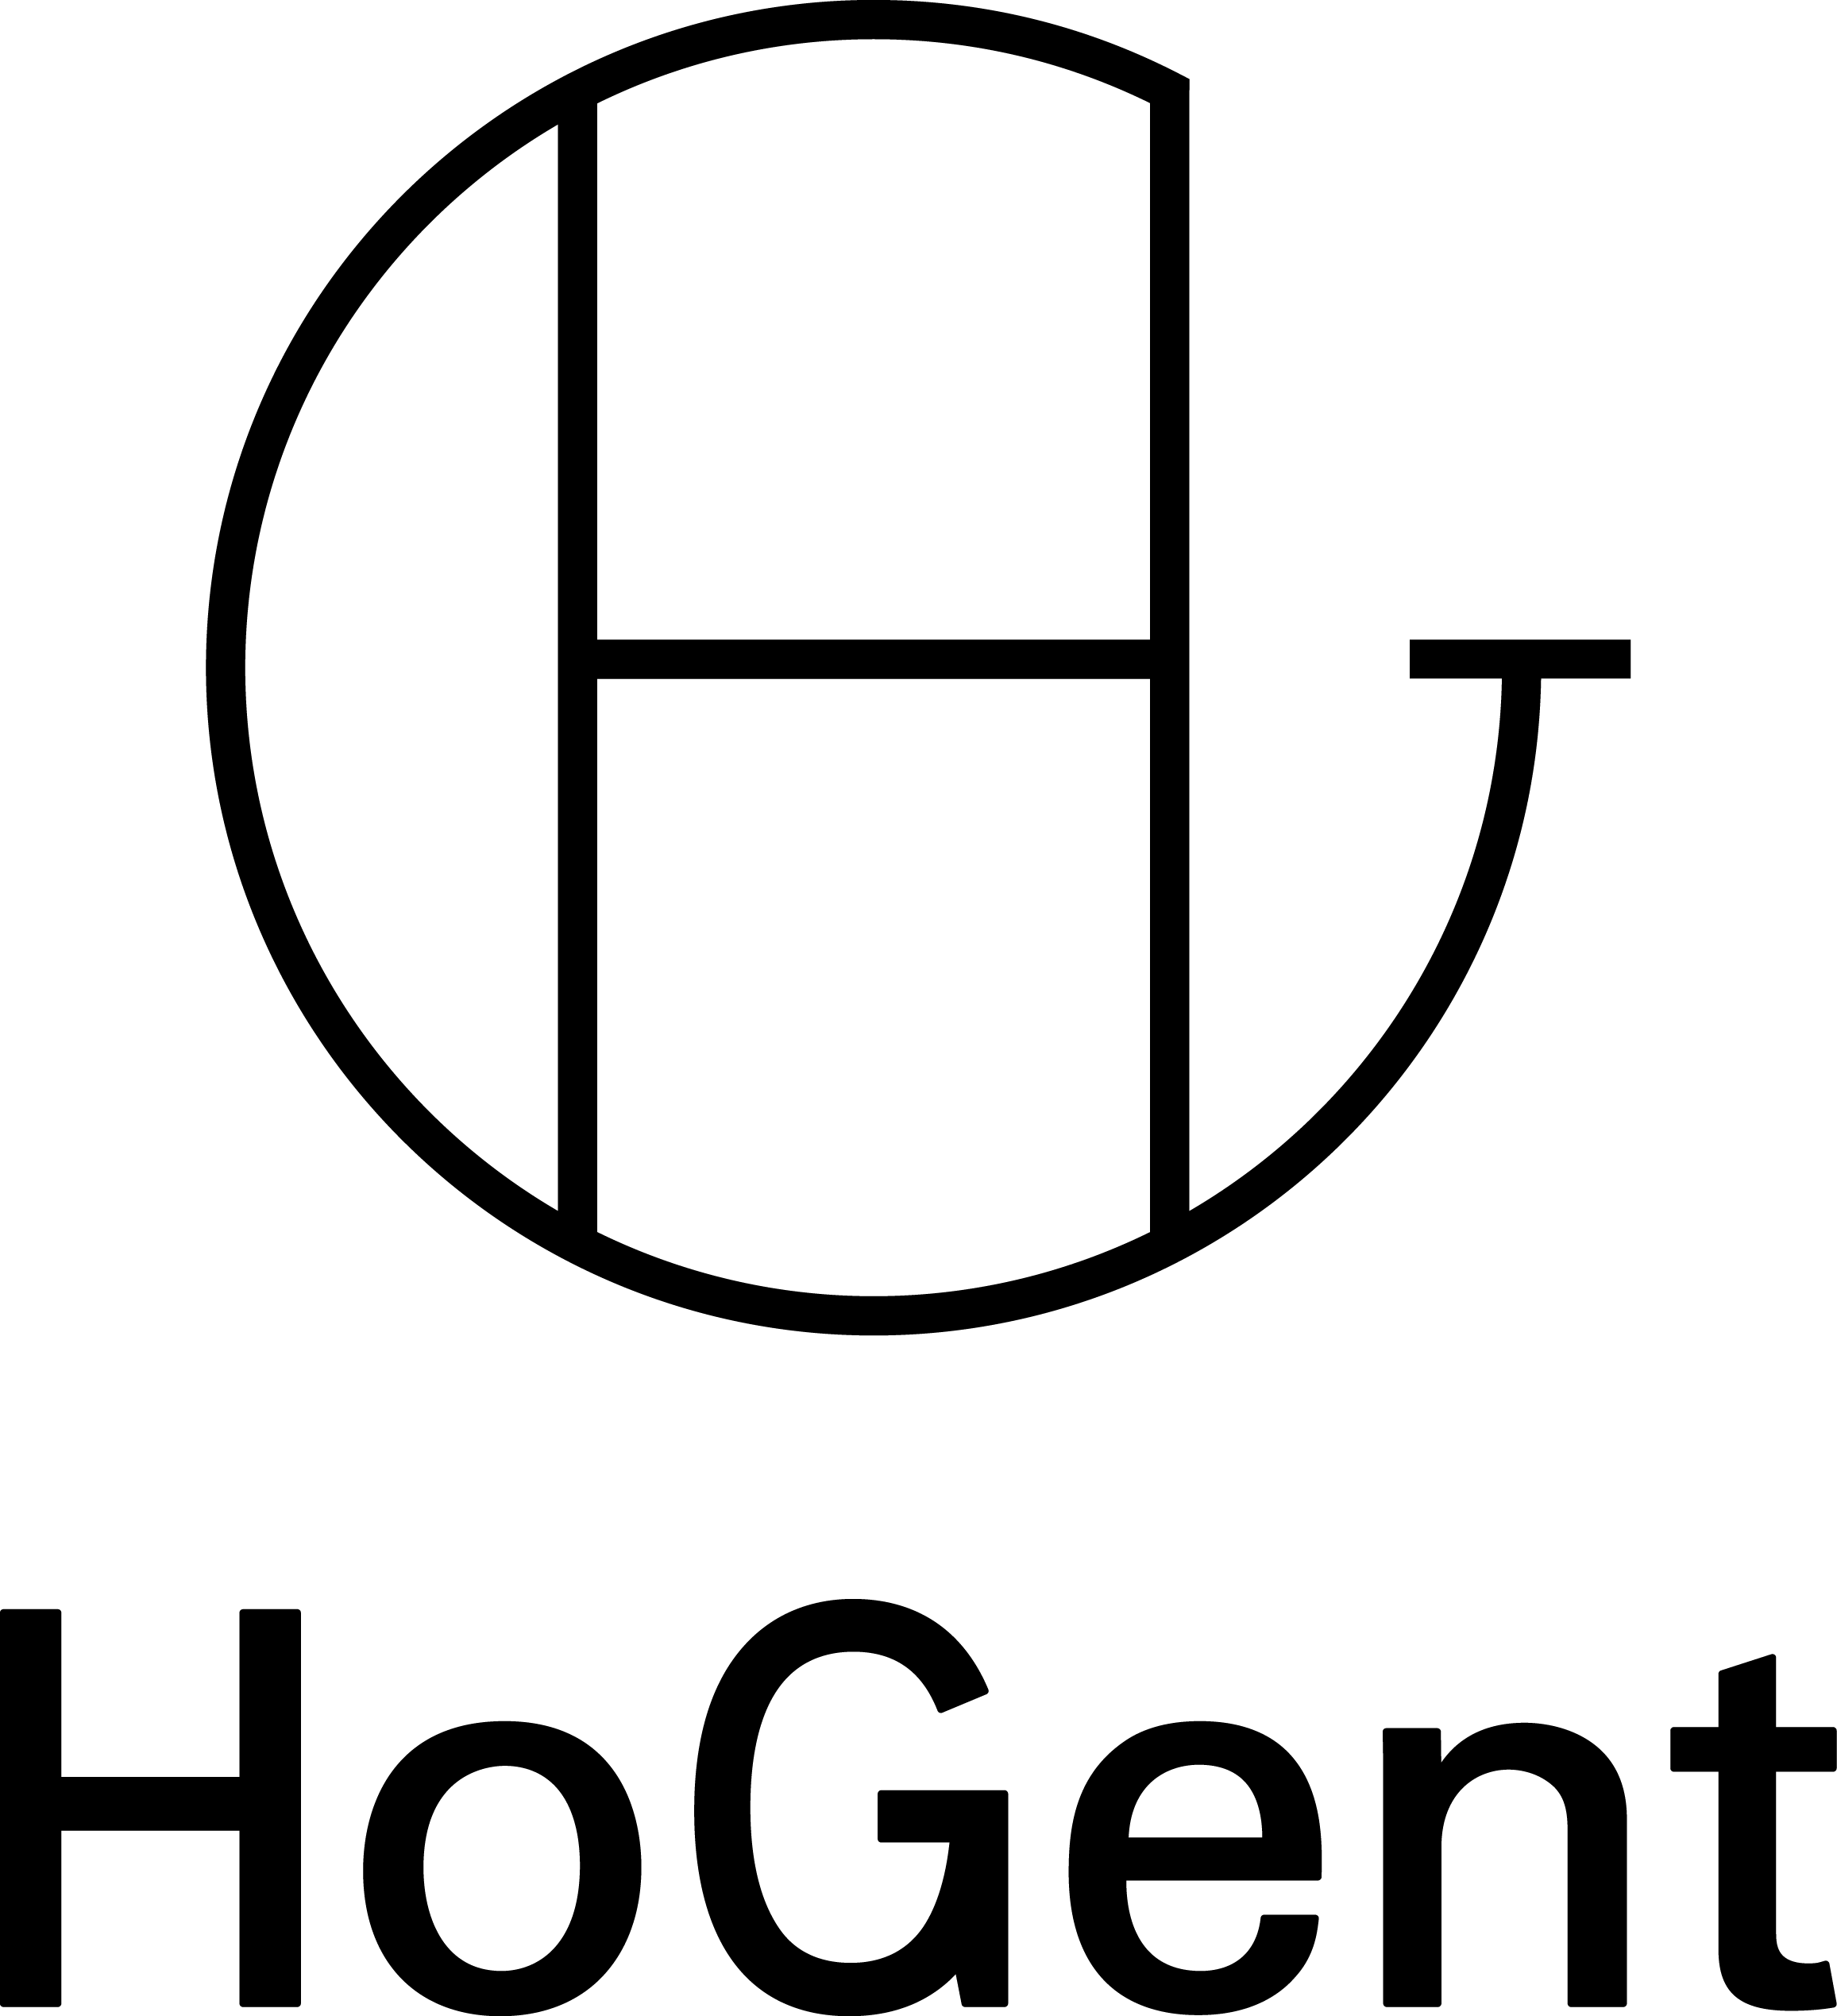
\includegraphics[width=2.5cm]{img/HG-beeldmerk-woordmerk}\\[.5cm]
    \faculteit\\[3cm]
    \titel
    \vfill
    \student\\[3.5cm]
    \rapporttype\\[2cm]
    Promotor:\\
    \promotor\\
    Co-promotor:\\
    \copromotor\\[2.5cm]
    Instelling: \instelling\\[.5cm]
    Academiejaar: \academiejaar\\[.5cm]
    \examenperiode
    \endgroup

  \end{center}
  \restoregeometry
\end{titlepage}

% Schutblad

\emptypage


\begin{titlepage}
  \newgeometry{top=5.35cm,bottom=1.5cm,left=1.5cm,right=1.5cm}
  \begin{center}

    \begingroup
    \rmfamily
    \faculteit\\[3cm]
    \titel
    \vfill
    \student\\[3.5cm]
    \rapporttype\\[2cm]
    Promotor:\\
    \promotor\\
    Co-promotor:\\
    \copromotor\\[2.5cm]
    Instelling: \instelling\\[.5cm]
    Academiejaar: \academiejaar\\[.5cm]
    \examenperiode
    \endgroup

  \end{center}
  \restoregeometry
\end{titlepage}


\begin{abstract}
% TODO: De "abstract" of samenvatting is een kernachtige (max 1 blz. voor een
% thesis) synthese van het document. In ons geval beschrijf je kort de
% probleemstelling en de context, de onderzoeksvragen, de aanpak en de
% resultaten.
Vandaag de dag hoor je regelmatig eens in het nieuws dat er een bedrijf is opgelicht door professionele hackers, oplichters die zijn binnen gedrongen in hun netwerk en gevoelige informatie hebben gebruikt om zaken te verkrijgen. Dit probleem groeit even snel als de groei van netwerken in het bedrijfsleven. Daarom is het belangrijk om een zeer goed beveiligd netwerk te hebben tegen bedreigingen van zowel binnen als buiten het bedrijf. \newline \newline

Mijn grootste doelstelling is om een overzicht te voorzien van welke soorten maatregelen er zeker moeten getroffen worden om een netwerk optimaal te beveiligen. Dit gaande van de router tot de switch tot de server. Ik wil zelf ook zo een beveiligd netwerk/server kunnen opzetten en zelf kunnen testen dat er geen enkele vorm van bekende bedreigingen binnen kan. Tot slot wil ik te weten komen of er in het bedrijfsleven wel nood en budget is voor zulke hevige beveiligingen. \newline \newline

Om dit probleem te onderzoeken heb ik op voorhand enkele onderzoeksvragen vastgesteld. Wat zijn de bekendste soorten van externe en interne bedreigingen en hoe worden deze het efficiëntst opgelost? Hoe word je router en switch zo optimaal mogelijk beveiligd? Hoe wordt de server zo goed mogelijk beveiligd? Wat zijn de voor -en nadelen van bepaalde beveiligingstechnieken? \newline 


\textbf{- Wat zijn de bekendste soorten van externe bedreigingen en hoe los je deze het efficiëntst op? - Wat zijn de bekendste soorten van interne bedreigingen en hoe los je deze het efficiëntst op? - Is er in het huidige bedrijfsleven (kleine, middelgrote en grote ondernemingen) nood/budget aan een stevige beveiliging. - Hoe beveilig je de router en switch zo optimaal mogelijk? - Hoe beveilig je de server en werkstations zo optimaal mogelijk? - Wat zijn de voor -en nadelen van bepaalde beveiligingstechnieken? .... 
} (KAN NOG VERANDEREN)
\end{abstract}

\chapter*{Voorwoord}
\label{ch:voorwoord}
Deze scriptie zou niet to stand gekomen zijn zonder de hulp van mijn stagementer en co-promotor Selami Top. Ik mocht gebruik maken van zijn huidig netwerk en ik mocht enkele zaken uitproberen op zijn nieuw netwerk. Hierdoor kon ik de zaken die ik onderzocht en opgezocht had uit proberen in een echte omgeving en kreeg ik een betere kijk op een realistische beveiliging. Verder wil ik ook mijn promotor Bert Van Vreckem bedanken die mij heeft geholpen om deze bachelorproef tot stand te brengen. (NOG WAT TOEVOEGEN). Tot slot wil ik alle auteurs bedanken van de lectuur die ik heb gebruikt om deze scriptie te maken (LIJST VAN ALLE AUTEURS?)
% TODO: Vergeet ook niet te bedankten wie je geholpen/gesteund/... heeft

\tableofcontents

% Als je een lijst van afkortingen of termen wil toevoegen, dan hoort die
% hier thuis. Gebruik bijvoorbeeld de ``glossaries'' package.

%%---------- Kern --------------------------------------------------------

\chapter{Inleiding}
\label{ch:inleiding}

De inleiding moet de lezer alle nodige informatie verschaffen om het onderwerp te begrijpen zonder nog externe werken te moeten raadplegen \citep{Pollefliet2011}. Dit is een doorlopende tekst die gebaseerd is op al wat je over het onderwerp gelezen hebt (literatuuronderzoek). \newline \newline

Je verwijst bij elke bewering die je doet, vakterm die je introduceert, enz. naar je bronnen. In \LaTeX{} kan dat met het commando \texttt{$\backslash${cite\{\}}} of \texttt{$\backslash${citep\{\}}}. Als argument van het commando geef je de ``sleutel'' van een ``record'' in een bibliografische databank in het Bib\TeX{}-formaat (een tekstbestand). Als je expliciet naar de auteur verwijst in de zin, gebruik je \texttt{$\backslash${}cite\{\}}.
Soms wil je de auteur niet expliciet vernoemen, dan gebruik je \texttt{$\backslash${}citep\{\}}. Hieronder een voorbeeld van elk.

\cite{Knuth1998} schreef een van de standaardwerken over sorteer- en zoekalgoritmen. Experten zijn het erover eens dat cloud computing een interessante opportuniteit vormen, zowel voor gebruikers als voor dienstverleners op vlak van informatietechnologie~\citep{Creeger2009}.

\section{Probleemstelling en Onderzoeksvragen}
\label{sec:onderzoeksvragen}

% TODO: Wees zo concreet mogelijk bij het formuleren van je
% onderzoeksvra(a)g(en). Een onderzoeksvraag is trouwens iets waar nog
% niemand op dit moment een antwoord heeft (voor zover je kan nagaan).
\subsection{Hoe kan port scanning de beveiliging van je eigen netwerk verbeteren en wat zijn de gevaren ervan?}

Port scanning is een bekende manier om iemand zijn netwerk in kaart te brengen en te kijken naar een manier hoe je er binnen kan geraken. Port scanning is kan jouw netwerk in gevaar brengen, maar kan er ook voor zorgen dat jouw netwerk beter beveiligd is als je weet hoe je het moet gebruiken en hoe je jezelf ertegen moet beschermen. De vraag die hier wordt gesteld is hoe dat je port scanning als ethische hacker kan gebruiken om jouw netwerk beter te beveiligen tegen mensen die port scannen gebruiken voor niet zo ethische doelstellingen.

\subsection{Wat is de beste en efficiënste manier om jouw netwerk te beschermen tegen port scanning?}

\chapter{Methodologie}
\label{ch:methodologie}

% TODO: Hoe ben je te werk gegaan? Verdeel je onderzoek in grote fasen, en
% licht in elke fase toe welke stappen je gevolgd hebt. Verantwoord waarom je
% op deze manier te werk gegaan bent. Je moet kunnen aantonen dat je de best
% mogelijke manier toegepast hebt om een antwoord te vinden op de
% onderzoeksvraag.
\section{Port scanning}
\subsection{Onderzoek}
Om een goed antwoord te kunnen geven op deze onderzoeksvraag moet ik eerst een goede kennis hebben over het onderwerp. Dit heb ik gedaan door het verzamelen van lectuur over hoe je moet ethisch hacken en wat port scanning precies is. Om de gevaren van port scanning te kennen, moet ik eerst weten hoe een port scan werkt en hoe ik de output ervan kan interpreteren. 

\subsection{Opzetten testomgeving}
Om zelf wat ervaring op te doen met port scanning ben ik gestart met een virtuele machine te maken waarop Windows Server 2012 R2 op geïnstalleerd staat. Als eerste heb ik deze domeincontroller gemaakt in het fictieve domein \textit{HARDO}. Verder heb ik ook de rollen DNS, DHCP en Externe toegang geïnstalleerd en heb ik al subnet gekozen voor 192.168.1.0/24 waar ik de range 192.168.1.1 tot 192.168.1.30 heb ik uitgesloten voor distributie. Daarna ben ik naar de website van nmap gegaan om de nmap-tools te downloaden. Deze zijn zeer belangrijk om zelf aan port scanning te doen. Tot slot heb ik de server het IP-adres 192.168.1.2 gegeven. \newline

Nu dat er 1 server opstaat is het tijd om enkele hosts op te zetten en deze toe te voegen aan het domein. Ik heb 3 Windows 8.1-hosts opgezet met de IP-adressen 192.168.1.31 - 192.168.1.32 - 192.168.1.33 en naam WS1 - WS2 - WS3. Met deze 4 virtuele machines kan ik verschillende soorten software en technologieën testen die ervoor zorgen dat ik mijn onderzoeksvragen zo nauwkeurig en correct mogelijk kan beantwoorden.

\subsection{}
\chapter{Port scanning interpreteren}

%% TODO: de structuur en titel van deze hoofdstukken hangen af van je
% eigen onderzoek. Elke fase in je onderzoek kan een eigen hoofdstuk krijgen. Kies telkens een gepaste titel. ``Corpus'' is *GEEN* gepaste titel

\section{Wat is port scanning?}
Om te antwoorden op de onderzoeksvragen moet je eerst weten wat port scanning precies is en doet. Port scanning is één van de meest gebruikte en bekendste manieren die er bestaat om een weg te vinden in het netwerk van een persoon of een bedrijf. Bij een port scan wordt er gekeken welke poorten er allemaal open staan in een netwerk. Via poorten wordt er informatie verzonden en ontvangen dus je kan deze techniek vergelijken met in een gang met 65 535 deuren aan elke deur eens voelen en kijken of deze open staat of gesloten is. \newline \newline

Door een port scan uit te voeren op een netwerk kan je zien welke poorten er open zijn, maar ook welke poorten er luisteren. Dit wilt zeggen welke poorten er informatie ontvangen. Je kan ook zien welke beveiligings apparaten zoals firewalls die aanwezig zijn tussen de zender en de ontvanger. Deze techniek wordt ook wel fingerprinting genoemd en wordt vaak gebruikt door aanvallers om een zwak punt in het netwerk te vinden. 

\section{Soorten port scans MEER INFO ZOEKEN}
Er zijn verschillende soorten port scans en elk van deze hebben hun eigen accenten. 
\begin{itemize}
	\item Vanilla = Ook wel een "full scan" genoemd. Hierbij wordt er geprobeerd om met alle 65 535 poorten verbinding te maken. Er wordt een SYN flag (vraag om te verbinden) verzonden en na het ontvangen van een SYN-ACK respons wordt er een ACK flag teruggestuurd. Dit staat ook wel bekend als een TCP handshake. Deze soort scans zijn zeer nauwkeurig maar zijn makkelijk detecteerbaar omdat deze soort verbindingen altijd worden gelogged door de firewall.
	\item Fragmented Packets = De scanner zend fragmenten van pakketten uit die door een simpele packet filter geraken in een firewall.
	\item Strobe = Is een iets specifiekere scan die enkel kijkt naar bekende services die kunnen geexploid worden.
	\item Stealth scan = De scanner blokkeert de gescande computer om de port scan activiteiten te onthouden.
	\item UDP = Er wordt gekeken naar open UDP-poorten.
	\item FTP Bounce = Scanner gaat door een FTP-server om de bron van de scan te verbergen.
\end{itemize}

\chapter{Port scanning als bedreiging}



\chapter{Port scanning als hulpmiddel}


\chapter{Conclusie}
\label{ch:conclusie}

% TODO: Trek een duidelijke conclusie, in de vorm van een antwoord op de
% onderzoeksvra(a)g(en). Reflecteer kritisch over het resultaat. Zijn er
% zaken die nog niet duidelijk zijn? Heeft het ondezoek geleid tot nieuwe
% vragen die uitnodigen tot verder onderzoek?
\lipsum[76-80]


\bibliographystyle{apa}
\bibliography{tin-bachproef}

%%---------- Back matter -------------------------------------------------

\listoffigures
\listoftables

\end{document}
